%%%%%%%%%%%%%%%%%%%%%%% file template.tex %%%%%%%%%%%%%%%%%%%%%%%%%
%
% This is a general template file for the LaTeX package SVJour3
% for Springer journals.          Springer Heidelberg 2010/09/16
%
% Copy it to a new file with a new name and use it as the basis
% for your article. Delete % signs as needed.
%
% This template includes a few options for different layouts and
% content for various journals. Please consult a previous issue of
% your journal as needed.
%
%%%%%%%%%%%%%%%%%%%%%%%%%%%%%%%%%%%%%%%%%%%%%%%%%%%%%%%%%%%%%%%%%%%
%
% First comes an example EPS file -- just ignore it and
% proceed on the \documentclass line
% your LaTeX will extract the file if required
\RequirePackage{fix-cm}
%
%\documentclass{svjour3}                     % onecolumn (standard format)
\documentclass[referee,natbib,smallcondensed]{svjour3}     % onecolumn (ditto)
%\documentclass[smallextended]{svjour3}       % onecolumn (second format)
%\documentclass[twocolumn]{svjour3}          % twocolumn
%
\smartqed  % flush right qed marks, e.g. at end of proof
%

%
% \usepackage{mathptmx}      % use Times fonts if available on your TeX system
%
% insert here the call for the packages your document requires
%\usepackage{latexsym}
% etc.
\usepackage{float,comment} %Personal
\usepackage{amsmath,amssymb,amsfonts,changes,todo} %Personal
%\usepackage[authoryear,sectionbib,sort]{natbib}
\usepackage{lineno,url}
\usepackage{graphics,epsfig} %Personal



\makeatletter
\let\cl@chapter\undefined
\makeatletter
\usepackage{cleveref} %Personal
%\usepackage{anyfontsize} %Personal
%\usepackage{changes}



% please place your own definitions here and don't use \def but
\DeclareMathOperator{\argmax}{argmax}
\DeclareMathOperator{\ess}{ess}

\newcommand{\pa}[1]{\left ( #1 \right )}
\newcommand{\abs}[1]{\left | #1 \right |}
\newcommand{\for}[0]{\text{ for }}
\newcommand{\osum}{\oplus}
\newcommand{\overbar}[1]{\mkern 1.5mu\overline{\mkern-1.5mu#1\mkern-1.5mu}\mkern 1.5mu}
\newcommand{\ip}[2]{\left \langle #1,#2 \right \rangle}
\newcommand{\brak}[1]{\langle #1 \rangle}
\newcommand{\N}[0]{\mathbb{N}}
\newcommand{\C}[0]{\mathbb{C}}
\newcommand{\Z}[0]{\mathbb{Z}}
\newcommand{\T}[0]{\mathcal{T}}
\newcommand{\R}[0]{\mathbb{R}}
\newcommand{\Q}[0]{\mathbb{Q}}
\newcommand{\B}[0]{\mathcal{B}}
\newcommand{\bra}[1]{\langle #1 \rvert}
\newcommand{\ket}[1]{\lvert #1 \rangle}

\newcommand{\norm}[1]{\left \Vert #1 \right \Vert }



\let\oldphi\phi \let\phi\varphi \let\varphi\oldphi
\let\oldphi\phi \let\epsilon\varepsilon

%
% Insert the name of "your journal" with
\journalname{Journal of Mathematical Biology}
%
\begin{document}


\title{Population games with instantaneous behavior and the Rosenzweig-MacArthur model
%\thanks{This work was supported by the Centre for Ocean Life,
%a Villum Kann Rasmussen Centre of Excellence supported
%by the Villum Foundation.}
}
%\subtitle{Do you have a subtitle?\\ If so, write it here}

\titlerunning{Population games with instantaneous behavior}        % if too long for running head

\author{Emil F. Fr{\o}lich
}

%\authorrunning{Short form of author list} % if too long for running head

\institute{Emil F. Fr{\o}lich \at
              Technical University of Denmark \\
              Department of Applied Mathematics and Computer Science - DTU Compute \\
              Building 303B, Matematiktorvet, Kgs. Lyngby \\
              Tel.: +45-26142497\\
              \email{jaem@dtu.dk}           %  \\
%             \emph{Present address:} of F. Author  %  if needed
}

\date{Received: date / Accepted: date}
% The correct dates will be entered by the editor


\maketitle
\newpage
\begin{abstract}
  Explaining spatial distribution and population dynamics of animals are some of the key questions in ecology. These two have been coupled before, but there has been no general method for determining spatial distributions. In particular, there is no general method for working with spatial distributions based on instantanous behavior coupled with population dynamics. We propose modeling interacting populations with instantaneous habitat choice through mean-field games. By using the framework of variational inequalities, we are able to determine existence and uniqueness for habitat distributions of interacting populations, in both continuous and discrete habitats. With some additional restrictions, we are also able to show existence and uniqueness of fixed-points of the population dynamics along with spatial distributions. We illustrate our theoretical results by studying a Rosenzweig-MacArthur model where predators and consumers inhabit a continuous habitat. We show existence and uniqueness of an instantaneous Nash equilibria for this model, and the existence and uniqueness of a fixed point of the model.
  The generality of our theoretical approach opens up for studying complex ecosystems, e.g. the impact of enrichment on spatial distributions in marine ecosystems.

\keywords{game theory, population dynamics, habitat choice, population game}
% \PACS{PACS code1 \and PACS code2 \and more}
% \subclass{MSC code1 \and MSC code2 \and more}
\end{abstract}

%Game theory has emerged as an important tool to understand interacting populations in the last 50 years. Game theory has been applied to study population dynamics with optimal behavior in simple ecosystem models, but existing methods are generally not applicable to complex systems. In order to use game-theory for population dynamics in heterogeneous habitats, habitats are usually split into patches and game-theoretic methods are used to find optimal patch distributions at every instant. However, populations in the real world interact in continuous space, and the assumption of decisions based on perfect information is a large simplification. Here, we develop a method to study population dynamics for interacting populations, distributed optimally in continuous space. A continuous setting allows us to model bounded rationality, and its impact on population dynamics. This is made possible by our numerical advances in solving multiplayer games in continuous space. Our approach hinges on reformulating the instantaneous game, applying an advanced discretization method and modern optimization software to solve it. We apply the method to an idealized case involving the population dynamics and vertical distribution of forage fish preying on copepods. Incorporating continuous space and time, we can model the seasonal variation in the migration, separating the effects of light and population numbers. We arrive at  qualitative agreement with empirical findings. Including bounded rationality gives rise to spatial distributions corresponding to reality, while the population dynamics for bounded rationality and complete rationality are equivalent. Our approach is general, and can easily be used for complex ecosystems.


\section{Introduction}

%Mention a few classic papers, mention the problem.
Game theory is a natural tool to model the behavior of animals, who must respond to the behavior of other animals as well as complex and rapidly shifting environments. A classical application of game-theory is patch-choice models, where the ideal free distribution emerges to explain spatial distributions  \citep{cressman2004ideal, fretwell1969territorial}. A game theoretical approach has been fruitful in studying habitat choice in simple ecosystems under the assumption of static populations or simplifying the habitat to a few discrete patches. Real-life habitat choice consists of animals choosing where to forage in a continuous landscape, with varying intra-specific competition and outside risk. Models that can handle such systems allow for better models of habitat distribution, and represent a significant step forward in understanding natural systems \citep{morris2003shadows}.

A common simplification when including behavior in population models is to assume that at least one payoff is linear in the choice of strategy, \citep{krivan1997dynamic}. Linear models are suffficient to explain simple predator-prey dynamics with optimal behavior, \citep{kvrivan2007lotka}, but non-linear effects in natural systems are substantial \citep{gross2009generalized}. A model for population games is set out in \citep{vincent2005evolutionary}.  Optimal behavior is introduced by every population maximizing the pr. capita growth at every instant. This implicitly assumes monomorphic populations, where all individuals intrinsically act as one \citep{malone2020ecology,stump2017optimally}. We propose a modification of the approach from \citep{vincent2005evolutionary} in the vein of \citep{cressman2010ideal}, based on individual optimization. Instead of assuming a population where all individuals act in lockstep, we assume that each animal acts independently, but that its risk-reward calculus is affected by the population mean behavior. This marks a return to the ideas of playing the field, \citep{smith1982evolution, cressman2010ideal}. If we assume large populations and that the animals of each type are indistinguishable, the game can be modeled as a static mean field game with multiple types.


The evolution of mean-field games has followed two parallel tracks, one in mathematical biology through the ideal free distribution \citep{fretwell1969territorial, cressman2004ideal, kvrivan2008ideal, cressman2010ideal, broom2013game, parker1978searching}, and the other in mathematical optimization based directly on anonymous actors \citep{lasry2007mean, aumann1964markets, blanchet2016optimal}. The main focus in ecology has been studying specific families of games in depth \cite{broom2013game}, while the focus in mathematical optimization has been in establishing uniqueness and existence of Nash equilibria through the toolbox of variational inequalities \citep{karamardian1969nonlinear, gabay1980uniqueness, nabetani2011parametrized}. We demonstrate that in certain cases, a mean-field game can be rephrased equivalently as a normal-form game. This allows us to bring the entire toolbox of variational inequalities to bear on population games.


Using the theory of variational inequalities, we show that population games based on individual optimization have a unique equilibrium under very general assumptions. Our approach allows us to handle both continuous and discrete strategy spaces, but more technical assumptions are required for existence in the continuous setting. The classical ideal free distribution emerges as a special case of our approach, providing a compelling argument for the mean-field approach. We demonstrate the fundamental difference between working with direct pr. capita optimization and using the mean field approach, explicitly quantifiying the difference in expected payoff for the case of the ideal free distribution. Behavior based on individual optimization appears more cautios than predicted when optimizing pr. capita consumption, which we demonstrate with an example and conjecture as a general property. We demonstrate our approach by applying it to a behaviorally modified Rosenzweig-MacArthur system in continuous space. We show that the system satisfies the criteria for existence and uniqueness as a population game.


In addition to our theoretical advances, we implement a simple and efficient numerical method of finding Nash equilibria and equilbria of population games. The approach is applied to our case of the behaviorally modified Rosenzweig-MacArthur system. We examine the population dynamics through a phase portrait, where they appear to be asymptotically stable. We study the population levels and spatial distribution at equilibrium as a function of the carrying capacity, intraspecific predator competition. The rest of the paper is organized as follows: We start with the general setting. After building the general setting, we introduce the machinery of variational inequalities in the context of game theory. Here we show the general uniqueness and existence results. We proceed to study the concrete Rosenzweig-MacArthur model, showing existence and uniqueness of the Nash equilibrium and population equilibrium. We analyze the results, and discuss the implications of both the results and our theoretical results.

%We illustrate the general theory with a behaviorally modified Rosenzweig-MacArthur system. We study the population dynamics in this system,  and the sensitivity of population levels and strategy distributions to the carrying capacity and intraspecific predator competition.

%Add references to krivan and cressmans other articles, including the empirical one by krivan.

%The study of population games through the ideal free distribution has had great success in the ecological litterature, but it has the weakness of being unable to handle games with non-linear interactions. Here we solve this problem by introducing results from the study of mean field games in mathematical optimization.


%In the study of habitat-choice games, the ideal free distribution is the correct choice, in contrast to full population optimization (cite monroe), with exceptions where inherently monomorphic populations are a resaonable assumption.
%The theory of population games has developed in the area of mathematical optimization, \citep{aumann} and mathematical biology simultaneously \citep{cressman,kvivran,etc}. In the field of mathematical optimization, it is typically described as static mean field game theory and is characterized by arriving at the ideal free distribution mathematical biology.

\section{Population games based on habitat choice}
\label{sec:general_setting}
We build the general setting piece-by-piece, from the environment to the foraging strategies. First we define the environment, then we introduce the mean-field setting, as it is necessary to handle the strategy of an entire population. With this in place, we can give an exact definition of a population game in our sense. Once we have laid the building blocks for our setting, we show that mean-field games generalize the ideal free distribution.


We envision a setting with $M$ different unstructured populations of animals co-existing in an environment, each with biomass $N_i$. We only model behavior as patch choice, excluding e.g. mating behavior. The distribution of population $i$ in the environment is described by $\overbar{\sigma}_i$.  More rigorously, we assume that the environment is a probability space $(X,\mu)$. Modeling the environment as a probability space allows us to model habitats which are continuous, discrete and mixtures thereof in the same context. As an example, bats forage over a continuous area while the caves where they rest are discrete and disconnected \citep{collet2019algorithmic}. We model that the populations $N_i$, $i\in \{1,\dots,M\}$  are large compared to a single individual. This allows us to consider the population as continuous, consisting of infinitely many individuals. We assume that the population dynamics depend both on the distributions and the population sizes:
\begin{equation}
  \label{eq:vk_dyn}
  \dot{N}_i = N_i f_i((N_j,\overbar{\sigma}_j)_{j=1}^M)
\end{equation}
That is, we consider population dynamics which can be described by a Kolmogorov model.

% so $N_i$ are continuous%, and so is the model. )% This allows us to model the population as continuous.ny
We suppose that the migration dynamics happen on a faster time-scale than the population dynamics, as is seen with e.g. vertical migrations in marine ecosystems \citep{iwasa1982vertical}. This slow-fast dynamic allows us to model the migrations as instantaneous, with each individual picking the optimal foraging ground at every instant \citep{kvrivan2013behavioral, cressman2006migration}.


We assume that every animal has an area where it forages at every instant. For an animal of type $i$ this is described by a probability distribution $\sigma_i$ over the environment $X$. We require that the distribution $\sigma_i$ is absolutely continuous with respect to the measure $\mu$. In an abuse of notation, we will denote this density by $\sigma$. We denote the space of probability densities over $X$ with respect to $\mu$ by $P_{\mu}$. We suppress $X$ for notational brevity. By requiring absolute continuity with respect to the base measure we remove degenerate Nash equilibria e.g. Dirac-type distributions in a continuous setting, avoiding for example all gazelles stacked exactly at a single point in space. We hereby generalize both the continuous and discrete approach to habitat selection \citep{fretwell1969territorial, broom2013game, verticalmigration}.


\subsection{Foraging strategies and mean-field}
In habitat choice games the essential choice an animal faces is where to forage, weighing risk and reward. Hence the density $\sigma_i$ describing where it forages is a strategic choice for an animal. As we assume instantaneous migrations and perfect information, an animal of type $i$ faces the foraging choices of all other inhabitants. Modeling the influence of the foraging choices necessitates the introduction of the mean-field-strategy, $\overbar{\sigma}_j$ for type $j$. The mean-field strategy $\overbar{\sigma}_j$ is the average strategy of all individuals of type $j$. As a consequence, we can describe the foraging presence from type $j$ at a point $x\in X$ by $N_j \overbar{\sigma}_j(x)$.

The choice of optimal foraging strategy $\sigma_i^*$ for an animal of type $i$ is a trade-off based on the presence of competitors, predators and prey. When considering animal populations, finding the optimal behavior for all individuals simultaneously quickly becomes infeasible. For this reason, we need to simplify the problem. This is where mean-field games come into play. The fundamental idea behind a mean-field game is that in a sufficiently large population, the decision of a single individual has no discernible on the average behavior of the population. In this case we can decouple the behavior of an individual and the mean behavior of the population, and assume that an individual plays against the average behavior of the population. That is, an individual plays the field \citep{smith1982evolution}. The fundamental assumption in the mean-field game that we consider is that the populations consist of infinitely many individuals acting instantaneously and independently so the choice of a single individual does not change the mean-field strategy \citep{aumann1964markets}


The mean density of competitors, predators and prey at a point $x$ is described by $N_j \overbar{\sigma}_j(x)$. We capture this trade-off for for each individual in a payoff function $U_i(\sigma_i, (N_j \overbar{\sigma}_j)_{j=1}^M)$. The payoff $U_i$ we have in mind is the instantanenous growth of an individual, i.e. individual fitness. This is given by the difference between the instantaneous per capita reproduction and mortality for an individual in \Cref{eq:vk_dyn}. When using the individual fitness as payoff, the Nash equilibria we find should be the same as simple ideal free distributions.
%Using the per capita growth as payoff, the Nash equilibrium becomes an evolutionarily stable state \citep{cressman2010ideal}.

Given that each type $j$ is distributed according to $\overbar{\sigma}_j$, the goal of a single animal of type $i$ is finding the optimal strategy $\sigma_i^*$ by playing the field at each instant such that
\begin{equation}
  \label{eq:ind_opt}
  \sigma^*_i = \argmax_{\sigma_i \in P_{\mu}} U_i(\sigma_i, (N_j, \overbar{\sigma}_j)_{j=1}^M)
\end{equation}
At the Nash equilibrium of a mean-field game every individual of type $i$ follows the same strategy $\sigma_i^*$, \citep{lasry2007mean, aumann1964markets}. Heuristically, this is due to interchangeability as if any individual of type $i$ gains by deviating from $\sigma_i^*$, any one of them would also gain from making the same deviation, hence doing so. Therefore, if they all follow the optimal strategy, they follow the same strategy. This allows us to go from the individual-level optimization to the Nash equilibrium in \Cref{eq:ind_opt}. %Considering $\sigma^*_{j}$ as a function of $\overbar{\sigma}_j$ the Nash equilibrium $\overbar{\sigma}_j^N$ for the mean-field game is the solution to the equation:
%\begin{equation}
%  \sigma^*_{j}(\overbar{\sigma}^N_j) = \overbar{\sigma}^N_j
%\end{equation}
Using $^N$ to denote the Nash equilibrium, the mean-field equilibrium $\overbar{\sigma}_i^N$ is the solution to the equation:
\begin{equation}
  \label{eq:mfg_ne}
  \overbar{\sigma}_i^N = \pa{\argmax_{\sigma_i \in P_{\mu}} U_i(\sigma_i, (N_j \overbar{\sigma}_j)_{j=1, j\neq i}^M, N_i \overbar{\sigma}_i^N) }
\end{equation}
Hence the Nash equilibrium of a game with $M$ interacting populations is the solution to the system of equations:
\begin{equation}
  \label{eq:tot_nash_eq}
  \begin{split}
    \overbar{\sigma}_1^N = \pa{\argmax_{\sigma_1 \in P_{\mu}} U_1(\sigma_1, (N_j \overbar{\sigma}^N_j)_{j=1}^M) } \\
    \vdots \\
    \overbar{\sigma}_M^N = \pa{\argmax_{\sigma_M \in P_{\mu}} U_M(\sigma_M, (N_j \overbar{\sigma}^N_j)_{j=1}^M) }
    \end{split}
\end{equation}
This system of equations looks intractable, but in the next section we will see that in many cases it can actually be solved using the toolbox of variational inequalities. Introducing \Cref{eq:tot_nash_eq} allows us to define a population game exactly.
%2) Polymorphic-Monomorphic equivalence
\begin{definition}\label{def:pop_game}
  A population game consists of $M$ unstructured populations with each population having a biomass of size $N_i$ with dynamics given by \Cref{eq:vk_dyn}. Each individual of type $i$ has a payoff function $U_i(\sigma_i,  (N_j \overbar{\sigma}_j)_{j=1}^M))$.  Migrations are instantanenous, and at every instant the populations are distributed according to the mean-field Nash equilibrium \Cref{eq:tot_nash_eq}, $\overbar{\sigma}_i^N$.
\end{definition
As noted, the example to keep in mind in \Cref{def:pop_game} is the example where the individual payoff $U_i$ functions are given by the fitness of an individual. The Nash equilibrium \Cref{eq:tot_nash_eq} in this case will correspond to the situation where all individuals of each type have the same fitness and do not gain from deviating, by \Cref{eq:tot_nash_eq}, i.e. the simple ideal free distribution \citep{fretwell1969territorial}. We repeat the caveat that this version of the ideal free distribution does not incorporate any stability criteria \citep{kvrivan2008ideal}. For this reason, we will generally refrain from using the terminology "the ideal free distribution" and instead always refer to \Cref{eq:tot_nash_eq} as the Nash equilibrium of a mean-field game. We will give a definition of the multi-species ideal free distribution once we have introduced the entire framework of variational inequalities and their coupling with Nash equilibria .

Though we focus on population games with the individual fitness as payoff function, an appeal of the mean-field approach is that it allows general payoff functions. As an example, the impact of cooperation in a spatially extended game can be investigated by using a mean-field approach \citep{Mean-field interactions in evolutionary spatial games}.


%Advantages of general approach:
%1) Easily generalizes IFD
\begin{comment}
\subsection{The ideal free distribution and mean-field games}
Assuming monomorphic populations is the typical approach to population games with instantaneous migrations  \citep{kvrivan2013behavioral, vincent2005evolutionary}, but it is well-known that this does not generalize the ideal-free distribution and dramatically increases the per capita gain \citep{kvrivan2008ideal}. We show that mean-field games generalize the classical ideal free distribution for single species, in the vein of \citep{cressman2010ideal}.
\begin{definition}[The ideal free distribution]
  Given a habitat $X$ with $M$ interacting species where an individual of type $i$ has a per capita-growth $U_i$. Assume each population is distributed according to $\overbar{\sigma}_i$. Further assume that the per capita growth is given by $\sigma$
\end{definition}
We start with a logistic population model where the density dependence is linear \cite{cressman2004ideal}. Afterwards, we show that mean-field games generalizing the ideal free distribution is a general phenomenon.
Before we proceed, we need to recall a simple version of the Karush-Kuhn-Tucker (KKT) conditions that we need. For the full version, see e.g. \citet{deimling2010nonlinear}.
\begin{theorem}
  A minimum $x^*$ of a Gateaux differentiable function $f$ in $P_{2,\mu} \subset L^2(X)$ satisfies the necessary condition that here exists an element $\nu \in H^+$ and a scalar $\lambda \in \R$ such that:
  \begin{equation}
    f(x^*) + \nu &= 1_H \lambda \\
    \ip{x^*}{\nu} &= 0
  \end{equation}
  The condition $\ip{x^*}{\nu} = 0$ is described as the complementary slackness conditions, and the requirements that $x^* \in P_{2,\mu}$, i.e. $x^* \geq 0$ and $\int x^* d\mu = 1$ are the primal conditions. The variable $\lambda$ is a Lagrange multiplier, and $\nu$ is typically referred to as a slack variable.
\end{theorem}
Consider a population of size $N$ and a discrete space $X$ with $L$ points, To emphasize the discrete nature, the strategy of an individual is denoted $p$ rather than $\sigma$ and the mean-field strategy then becomes $\overbar{p}$. We assume the population dynamics are governed by the logistic equation:
\begin{equation}
  \dot{N} = N\ip{\overbar{p}}{b} - N^2 \ip{\overbar{p}}{A\overbar{p}}
\end{equation}
where the $L\times L$ matrix $A$ encapsulates the density dependence the vector $b$ gives the spot-wise payoff. Hence the the first term $\overbar{p}{b}$ represents the growth from individuals foraging, and the second term $N^2 \ip{\overbar{p}}{A\overbar{p}}$ represents the density-dependent loss. The instantanous growth of an individual playing the strategy $p$ then becomes:
\begin{equation}
  \label{eq:mfg_simple}
  U(p,\overbar{p}) = \ip{p}{b} - N \ip{p}{A\overbar{p}}
\end{equation}
By considering $U$ as a payoff function, we can consider the mean-field game at every instant where every individual seeks to optimize $U(p,\overbar{p})$. Denote the Nash equilibria of the mean-field game defined by \Cref{eq:mfg_simple} by $p^N$.
\begin{proposition}
  \label{prop:doubleup}
  The Nash equilibrium $\overbar{p}^{N}$ for the game defined by \Cref{eq:mfg_simple} is the ideal free distribution.
\end{proposition}
\begin{proof}
Consider the payoff in the mean-field situation $U(p,\overbar{p})$.
\begin{align}
  U(p, \overbar{p}) = N \ip{p}{A\overbar{p}}
\end{align}
Using the KKT conditions and defining $1_{\R^L}$ as a vector with $L$ ones, we can write up the requirements for an extremum $p^{N}$. The Lagrange multiplier $\lambda$ comes from the constraint that $p$ is a probability vector, and the complementarity slackness $\nu$ comes from the non-negativity of $p$.
\begin{equation}
  \begin{split}
    N \cdot A\overbar{p} + b + \nu = \lambda e \\
    \ip{p}{\nu} = 0 \\
    \nu \geq 0,~p \geq 0 \\
    \sum_{j=1}^L p^{j} = 1
  \end{split}
\end{equation}
As we are in the mean-field case, at the Nash equilibrium $p = \overbar{p} = \overbar{p}^N$ \Cref{eq:mfg_ne}.
so we can insert $\overbar{p}^N$ in the KKT conditions, to get:
\begin{equation}
  \begin{split}
    \label{eq:kkt_applied}
    N \cdot A\overbar{p}^N + b + \nu =  \lambda e \\
    \ip{\overbar{p}^N}{\nu} = 0 \\
    \nu \geq 0,~\overbar{p}^N \geq 0 \\
    \sum_{j=1}^L \overbar{p}^{N,j} = 1
  \end{split}
\end{equation}
The first equation ensures that $N\cdot A\overbar{p}^N + b + \nu$ is constant. At the same time, $\overbar{p}^N=0$ whenever $\nu > 0$ due to the second equation. Hence $N\cdot A\overbar{p}^N + b$ is constant, and equals $\lambda$. For any $j$ where $(N\cdot A\overbar{p}^N)_j$ would be less than $\lambda$, the value of $\overbar{p}^N_j$ is zero.
These are exactly the criteria for the ideal free distribution \citep{fretwell1969territorial}, illustrating the ideal free distribution as a special case of a mean-field game.
\qed
\end{proof}
%That is, assuming a monomorphic population doubles the payoff at the Nash equilibrium.
In \Cref{prop:doubleup} the ideal free distribution emerges as the mean-field equilibrium for a game with an affine payoff.
\begin{proposition}
  \label{prop:doubleup}
  Given a game
\end{proposition}
The emergence of the ideal-free distribution is a compelling argument for the mean-field model for modeling population games. In \Cref{prop:doubleup} we only considered a bilinear density dependence to give a better intuition. The proof, however, goes through for general non-linear functions of density dependence \citep{fretwell1969territorial} as the crux of the proof is recognizing that the KKT conditions for the payoff function $U(\sigma,\overbar{\sigma})$ are exactly the criteria for the ideal free distribution when imposing $\sigma = \overbar{\sigma}$ on the extrema as in \Cref{eq:kkt_applied}. We will return to

\begin{comment}
\begin{example}
  If we go back to the model in \Cref{prop:doubleup} and denote the identity matrix on $\R^n$ by $I_n$. Assume that $A=-I_2$ $b=(2,1)$ then assuming a monomorphic population leads to a dramatic increase in fitness and a different distribution compared to the mean-field approach. Assuming a monomorphic population in \Cref{prop:doubleup}, the payoff function is affine-quadratic $U(p,N p) = N \ip{p}{Ap} + \ip{b}{p}$.

\end{example}
In comparison, \Cref{prop:doubleup} shows that assuming a monomorphic population doubles the payoff compared to the ideal free distribution. This shows that the selflessness of an individual from assuming a monomorphic population is not insignificant, even in simple models.
\end{comment}

\section{Nash equilibria and variational inequalities}
Calculating Nash equilibria, \Cref{eq:tot_nash_eq} is generally a hard problem. A fruitful approach to calculating Nash equilibria is via. the theory of complementarity problems and variational inequalities \citep{karamardian1969nonlinear,nabetani2011parametrized}. We unite the approach of variational inequalities and mean-field games which allows us to characterize a situation that guarantees uniqueness and existence of Nash equilibria in population games, and the existence of fixed-points of these games.

%We develop the theory for monomorphic games, and finally introduce a method to analyze a mean-field game as a monomorphic game.

As in \Cref{sec:general_setting}, our habitat is a measure space $(X,\mu)$. We have $M$ different animal types coexisting with payoff-functions $U_i$. The simplest example our framework needs to handle is that of a single type with population $N$ inhabiting $X$ with following a distribution with density $\sigma$. The encounter rate of an individual following the strategy $\sigma$ with the entire population also following the strategy $\sigma$ is $N\sigma^2$. The expected total encounter for an individual with its conspecifics is
\begin{equation}
  N\int_X \sigma^2 d\mu
\end{equation}
and this quantity must be finite. This shows that the appropriate setting for our work is the space $L^2(X)$.
\begin{definition}
  Define the real Hilbert space $H=L^2(X)$, where $X$ is a measure space. Define $H_+ \subset H$ as the a.e. positive functions in $H$.
\end{definition}

\subsection{From Karush-Kuhn-Tucker to complementarity}
In order to find the Nash equilibrium of a population game, we need to solve \Cref{eq:tot_nash_eq}. We recall the setup of the $M$-player mean field game, now restricted to $H$. Assume we have $M$ different types of animals, with payoff functions $U_i$, and strategies $\sigma_i$, with corresponding mean-field strategies $\overbar{\sigma}_i$.
The Nash equilibrium of the game specified by the family $(U_i)$ corresponds to finding a system $\sigma_i^*$ satisfying the KKT conditions simultaneously for every $U_i$, \citep{deimling2010nonlinear}, with $\overbar{\sigma}=\sigma$ as in \Cref{eq:mfg_ne}. Denoting the identity on $H$ by $1_H$, the total criterion for a Nash equilibrium of a mean-field game \Cref{eq:tot_nash_eq} is:
\begin{equation}
      \label{eq:KKT_total}
  \begin{split}
  \begin{pmatrix}
    \nabla_{\sigma_1} U_1 \mid{\sigma_1 = \overbar{\sigma}_1} \\
    \vdots \\
    \nabla_{\sigma_N} U_N \mid{\sigma_N = \overbar{\sigma}_N}
\end{pmatrix} + \begin{pmatrix}
    \mu_1 \\
    \vdots \\
    \mu_N
\end{pmatrix} + \begin{pmatrix}
    \lambda_1 \cdot 1_k \\
    \vdots \\
    \lambda_N \cdot 1_k
\end{pmatrix} = 0 \\
\ip{
\begin{pmatrix}
  \mu_1 \\
  \vdots \\
  \mu_N
\end{pmatrix}}{ \begin{pmatrix}
  \sigma_1 \\
  \vdots \\
  \sigma_N
\end{pmatrix}} = 0 \\
\mu_i \in H_+ \\
  \sigma_i \in H_+ \\
  \int \sigma_i d\mu = 1
    %\sigma \in P_{2,\mu}(X)
  \end{split}
\end{equation}
Remark that the last two conditions are equivalent to $\sigma \in P_{\mu} \cap H$. This motivates the definition:
\begin{definition}
  Assume we have a measure space $(X,\mu)$. Consider the space of square-integrable functions $H=L^2(X,\mu)$ and space $P_{\mu}$ of probability densities over $X$. Define the space $P_{2,\mu}=H \cap P_{\mu}$ consisting of square-integrable probability densities.
\end{definition}
Solving the system in \Cref{eq:KKT_total} is highly non-trivial, but it turns out that reinterpreting the problem is helpful.
Finding Nash equilibria by interpreting the problem as a complementarity problem is one of the the original solutions to the hardness of finding Nash equilibria  \citep{karamardian1969nonlinear}. It turns out that the set of equations in \Cref{eq:KKT_total} is very close to being a complementarity problem, but first we need to introduce the notion.
\begin{definition}
  \label{def:comp_prob}
  Let $H$ be a real Hilbert space, and $K \subset H$ be a closed convex cone. Define $K^* = \{ x \in H : \ip{x}{y} = 0, \quad \forall y\in K\} $. Assume $T:K \to H$. The complementarity problem $CP(T,K)$ is the problem of finding an element $x$ such that
  \begin{equation}
    \begin{split}
    \ip{x}{Tx} = 0 \\
    Tx \in K^*, \quad  x\in K
  \end{split}
  \end{equation}
\end{definition}
With \Cref{def:comp_prob} we can write \Cref{eq:KKT_total} as an equivalent family of complementarity problems. Introduce $K = H_+ \osum \R$, with $K^* = H_+ \osum \{0\}$ and define
\begin{equation}
  T(\sigma_i, \lambda) = (-\nabla_{\sigma_i} U_i \mid{\sigma_i = \overbar{\sigma}_i} - \lambda_i \cdot 1_H, 0)
\end{equation}
Then the equations in \Cref{eq:KKT_total} can be recast as finding $(\sigma_i,\lambda_i) \in K$ such that:
\begin{equation}
  \label{eq:comp_form}
  \begin{split}
    \ip{T}{(\sigma_i,\lambda_i)} = 0 \\
    T((\sigma_i,\lambda_i) \in K^*
  \end{split}
\end{equation}
Or, equivalently:
\begin{equation}
  \begin{split}
    \ip{\sigma_i}{-\nabla_{\sigma_i} U_i \mid{\sigma_i = \overbar{\sigma}_i} - \lambda_i \cdot 1_H} + \ip{\lambda_i}{0}= 0 \\
    \pa{-\pa{\nabla_{\sigma_i} U_i \mid{\sigma_i = \overbar{\sigma}_i} - \lambda_i \cdot 1_H}, 0} \in K
  \end{split}
\end{equation}
There are dedicated tools available allowing for fast numerical resolution of complementarity problems \citep{acary2019introduction, dirkse1995path}. There is still the problem of establishing existence and uniqueness of the solution to this complementarity problem, which is generally hard, \citep{hadjisavvas2006handbook}.


%If $K$ is a convex cone, the problems $VI(T,K)$ and $CP(T,K)$ have the same solutions, which can be seen by setting $y=2x$ and $y=0$ respectively.

%To motivate the approach based on complementarity and variational inequalities,

%To put the problem of finding the Nash equilibrium into the terms of a complementarity problem, we generalize the strategy of \Cref{prop:doubleup}.
\begin{comment}
\begin{equation}
  \begin{split}
  \nabla_{\sigma_i}U_i((\sigma_j)_{j=1}^M) \mid_{\sigma_i = \overbar{\sigma}_i}  + \mu_i - \lambda  \cdot 1_H = 0 \\
  \ip{\sigma_i}{\mu_i} = 0 \\
  \mu_i \in H_+ \\
  \sigma_i \in H_+ \\
  \int_X \sigma_i d\mu(x)- 1 = 0
\end{split}
\end{equation}
\end{comment}
%Thus the condition for the Nash equilibrium of the total population as in \Cref{eq:tot_nash_eq} is:
\begin{comment}
The family of complementarity problems in \Cref{eq:comp_form} can be gathered into a single complementarity problem. We define $dU = \begin{pmatrix} \nabla_{\sigma_1} U_1 \mid_{\sigma_1 = \overbar{\sigma}_1}\\
    \vdots \\
    \nabla_{\sigma_N} U_N \mid_{\sigma_N = \overbar{\sigma}_N} \end{pmatrix}$, $S=(\sigma_i)_{i=1}^M$, and $\Lambda = (\lambda_i)_{i=1}^M$. Then \Cref{eq:KKT_total} can be restated as
\begin{equation}
  \label{eq:complementarity_form}
  \ip{dU(S)+\Lambda}{S} = 0 \\
  \ip{S_i-1}{1}\Lambda = 0
  -dU(S)-\Lambda \geq 0 \\
  \ip{S_i-1}{1} \in \{0 \}
  S\geq 0
  \Lambda \in \R^M
\end{equation}
which is a complementarity problem with $K = (H_+ \osum \R)^M$, $K^* = (H_+ \osum \{0\})^M$ and
\begin{equation}
  T(S,\lambda)=\begin{pmatrix} dU(S) + \Lambda \\ (\ip{\sigma_i}{1} - 1)_{i=1}^M \end{pmatrix}
\end{equation}
\end{comment}
\subsection{Restatement as a variational inequality}
We have recast the problem of finding a Nash equilibrium to a complementarity problem, which allows for numerical resolution. To establish existence and uniqueness, we need to use the relationship between complementarity problems and variational inequalities. We will show that in case the payoff-functions $U_i $ are sufficiently nice, the machinery of variational inequalities can be applied to show existence and uniqueness of the Nash equilibrium.

%Asking for convexity is too strong, but it turns out the weaker notion of strict pseudoconvexity is sufficient. See \Cref{sec:appendix} for further details.
We define a variational inequality:
\begin{definition}
  Let $H$ be a real Hilbert space and $K\subset H$ be a non-empty convex subset of $H$. Let $T: K \to H$. The variational inequality $VI(T,K)$ is the following system
  \begin{equation}
    x \in K, \ip{y-x}{Tx} \geq 0, \quad \forall y \in K
  \end{equation}
\end{definition}
The relationship between variational inequalities and complementarity problems is captured in \citep[Proposition 12.1]{hadjisavvas2006handbook}:
\begin{proposition}
  Let $K\subset H$ be a convex cone, and $T: K \to H$. Then the variational inequality $VI(T,K)$ is equivalent to the complementarity problem $CP(T,K)$.
\end{proposition}
\begin{proof}
  and a solution is an $x$ satisfying the inequality.
  Clearly, a solution $x^*$ to $CP(T,K)$ is also a solution to $VI(T,K)$. For the other direction, assume that we have a solution $x^*$ to VI(T,K). Then
  \begin{equation}
    \ip{y - x^*}{Tx^*} \geq 0 \forall y \in K
  \end{equation}
  Setting $y = 2x^*$, we arrive at $\ip{x^*}{Tx^*} \geq 0$, and setting $y=0$ we arrive at $\ip{x^*}{Tx^*} \leq 0$. This shows the desired equivalence.
\end{proof}
We can now turn the problem finding a Nash equilibrium into a variational inequality. Consider the problem as stated in \Cref{eq:comp_form}. This is a complementarity problem over the convex cone $H_+ \osum \R$. Hence it is equivalent to a variational inequality over the same convex cone with $T$ as in \Cref{eq:comp_form}
\begin{equation}
  \ip{T}{(\sigma_i' -\sigma_i,\lambda_i'-\lambda_i)} \geq 0, \quad \forall (\sigma_i', \lambda_i') \in K
\end{equation}
Since the second coordinate of $T$ is identically zero, this is the same as finding $(\sigma,\lambda)$ such that
\begin{equation}
  \label{eq:simp_var_eq}
  \ip{-\nabla_i U_i \mid_{\sigma_i = \overbar{\sigma}_i} - \lambda_i}{\sigma_i' -\sigma_i} \geq 0 \quad \forall \sigma_i' \in K
\end{equation}
In our theoretical considerations, we want to rid ourselves of the term $\lambda_i$, which stems from the constraint $\int_X \sigma_i d\mu = 1$. Hence solving \Cref{eq:simp_var_eq} over $K$ is equivalent to solving the constrained problem:
\begin{equation}
  \ip{-\nabla_i U_i \mid_{\sigma_i = \overbar{\sigma}_i}}{\sigma_i' -\sigma_i} \geq 0, \quad \sigma_i' \in P_{2,\mu}
\end{equation}
We can now state the problem of finding the Nash equilibrium \Cref{eq:tot_nash_eq} as finding the solution of a variational inequality.
\begin{definition}[Nash equilibrium as variational inequality]
  \label{def:var_eq_nash}
  Defining
\begin{equation}
  dU = \begin{pmatrix} \nabla_{\sigma_1} U_1 \mid_{\sigma_1 = \overbar{\sigma}_1}\\
      \vdots \\
      \nabla_{\sigma_N} U_N \mid_{\sigma_N = \overbar{\sigma}_N} \end{pmatrix}
\end{equation}
the problem of determining the Nash equilibrium \Cref{eq:tot_nash_eq} is the variational inequality of finding a vector $S = (\sigma_i)_{i=1}^M$ such that:
\begin{equation}
  \ip{-dU(S)}{W-S} \geq 0 \quad \forall W\in P_{2,\mu}^M
\end{equation}
\end{definition}
%i.e. solves a variational inequality. %Searching for a solution to a variational inequality is more tractable for theoretical considerations, while the complementarity formulation is preferable for solving the problem numerically.

%In case the payoff-functions $U_i $ are sufficiently nice, the machinery of variational inequalities can be applied to show existence and uniqueness of the Nash equilibrium. Asking for convexity is too strong, but it turns out the weaker notion of strict pseudoconvexity is sufficient. See \Cref{sec:appendix} for further details.
We need to introduce a specific type of variational inequality, which generalizes strict monotonicity of an operator, before we can state and prove a general theorem for uniqueness of the Nash equilibrium.
\begin{definition}
  \label{def:strict_pm}
 The operator $T: K \to H$ is strictly pseudomonotone if for every pair $x\neq y$ we have
 \begin{align}
   \ip{x-y}{Ty} \geq 0 \Rightarrow \ip{x-y}{Tx} > 0
 \end{align}
\end{definition}
With \Cref{def:strict_pm} in hand, we can finally give sufficient criteria for existence and uniqueness of the Nash equilibrium of the game specified in \Cref{eq:tot_nash_eq}.
\begin{theorem} \label{thm:nash_unique}
  Consider a game with $M$ players with payoff functions $U_i$ where each $-\nabla_{\sigma_i} U_i \mid_{\sigma_i = \overbar{\sigma}_i}$ is strictly pseudomonotone. Assume the strategies $\sigma_i$ are in $P_{2,\mu}$. The game has a unique Nash equilibrium if $dU$ as in \Cref{def:var_eq_nash} satisfies the criterion of \Cref{thm:existence} or $H$ is finite dimensional.
\end{theorem}
\begin{proof}
   If each $\nabla_{\sigma_i} U_i \mid_{\sigma_i = \overbar{\sigma}_i}$ is strictly pseudomonotone, then so is $dU$ by bilinearity of the inner product. By \Cref{thm:uniqueness} any Nash equilibrium will be unqiue since $dU$ is strictly pseudomonotone. So if the solution exists, it is unique. By assumption \Cref{thm:existence} gives existence of a solution of $VI(dU,P_{2,\mu}^M)$ in case $H$ is infinite dimensional. If $H$ is finite-dimensional then $P_{2,\mu}^M$ is compact and there exists a solution \Cref{rem:weak_compact}. \qed
\end{proof}
As a consequence of \Cref{thm:nash_unique}, we can introduce an equilibrium between the Nash equilibria of a mean-field game and a game with monomorphic populations.
%If the payoff functions ¤U_ mean-field game has a family of functions $U_i^{mon}$ satisfying $\nabla_{\sigma_i} U_i\mid{\sigma_i = \overbar{\sigma}_i} = \nabla_{\sigma_i} U_i^{mon}$, then the monomorphic game defined $U_i^{mon}$ has the same Nash equilbria as the original game.
\begin{definition}
  \label{def:correspondence}
  Consider a mean-field game with populations $N_1,\dots,N_M$ with individual payoffs $U_i(\sigma_i, (N_j \overbar{\sigma}_j)_{j=1}^M)$. Assume $\nabla_{\sigma_i}U_i\mid_{\sigma_i=\overbar{\sigma}_i}$ admits a primitive $U_i^{mon}$ such that $\nabla_{\sigma_i} U_i\mid{\sigma_i = \overbar{\sigma}_i} = \nabla_{\sigma_i} U_i^{mon}$.
   We define the monomorphic equivalent game as the game with monomorphic populations specified by the payoff functions $U_i^{mon}$.
\end{definition}
The reason this result is interesting is
\begin{theorem}[Theorem 12.13, p. 521 \citep{hadjisavvas2006handbook}]
  Let $\Omega \subset H$ be an open convex subset, and let $f:\Omega \to \R$ be Gateaux differentiable. Then $f$ is strictly pseudoconvex if and only if $\nabla f$ is strictly pseudomonotone.
\end{theorem}
so for uniqueness instead of considering $-\nabla U_i \mid_{\sigma_i = \overbar{\sigma}_i}$ we can consider $-U_i$ directly. That is, if a monomorphic equivalent game exists, it becomes possible to study the monomorphic game instead and use strict pseudoconvexity to establish strict pseudomonotonicity.
 %showing strict pseudoconvexity can be simpler than showing strict pseudomonotonicity.

With \Cref{thm:nash_unique}, we can show that there exist unique fixed points of population games where $dU$ is strictly pseudomonotone, e.g. if all monomorphic equivalent payoff functions are strictly pseudoconvex and bounded dynamics.
\begin{theorem}
  \label{thm:pop_game_exists_unique}
  We have a population game with $M$ populations of size $N_i$, payoff functions $U_i(\sigma_i, (N_j \overbar{\sigma}_j)_{j=1}^M)$ and dynamics given by $f_i(N_j \overbar{\sigma}_j)_{j=1}^M))$:
  \begin{equation}
    \dot{N_i} = N_i f_i
  \end{equation}
  Assume that the functions $f_i$ are strictly pseudomonotone, and that the set of stationary points of the dynamics is uniformly bounded in $(\sigma_i)_{i=1}^M$ and convex. Let $\nabla_{\sigma_i} U_i \mid_{\sigma_i = \overbar{\sigma}_i}$ be strictly pseudomonotone and satisfy \Cref{thm:existence}. Then the population game has a unique fixed point with a unique Nash equilibrium
\end{theorem}
\begin{proof}
  The game specified by the family $(U_i)_{i=1}^M$ has a unique Nash equilibrium for each $x\in \R^M$, given by a variational inequality problem over $P_{2,\mu}^M$ with operator $-dU$. The solution operator is a continuous mapping $G: \R_+^M \to P_{2,\mu}^M$, due to the existence and uniqueness of the solution \Cref{thm:nash_unique} \cite[Theorem 4.2]{barbagallo2009continuity}. The variational inequality defined by $(f_i)_{i=1}^M$ corresponds to determining fixed points. Due to the assumptions on $f_i$, this inequality has a solution $F$ for every family $(\sigma_i)_{i=1}^M$. The solution function $F:P_{2,\mu}^M: \to \R^M_+$ is again continuous.

  Finding a fixed point of the dynamical system along with a Nash equilibrium then corresponds to finding a fixed point of $F\circ G: \R_+^M \to \R_+^M$. Since the set of stationary points is assumed bounded, $G$ has compact range, and $F\circ G$ has compact image. Therefore $F\circ G:\R_+^M \to \R_+^M$ has a fixed point $(x_1^*, \dots, x_m^*)$ by Schauder's fixed point theorem \citep[Theorem 3.2, p. 119]{granas2003elementary}. Likewise, the map $G\circ F:P_{2,\mu}^M \to P_{2,\mu}^M$ has a fixed point $(\sigma_1^*,\dots, \sigma_M^*)$, since it factorizes through a compact space.
  For uniqueness, note that for each $(\sigma_i)_{i=1}^M$, the variational inequality
  \begin{equation}
    x \in \R_+^M, \ip{(f_i(x))_{i=1}^M}{y-x}\geq 0 \quad y\in \R_+^M
  \end{equation}
  has a unique solution, by strict pseudomonotonicity of $f_i$. If we append the two operators $(f_i)_{i=1}^M$ and $dU$ we get a single strictly pseudomonotone variational inequality, where the solution is unique.
   Therefore the simultaneous problem
  \begin{equation}
    \begin{split}
    S\in P_{2,\mu}^M, \ip{-dU(S))}{S'-S} \geq 0, \quad S' \in P_{2,\mu}^M \\
    x \in \R_+^M, \ip{(f_i(x))_{i=1}^M}{y-x}\geq 0 \quad y\in \R_+^M
  \end{split}
  \end{equation}
    has a unique solution, showing the existence and uniqueness of a fixed point for a population game.
    \qed
\end{proof}
%Remark that the assumption of uniformly bounded fixed-point space as a function of the strategies is biologically reasonable. As an example, if we consider a Type II functional response with clearance rate depending on the strategy and a constant metabolic loss.

Having established the general theory for Nash equilibria, and demonstrated how to handle mean-field games as monomorphic games, we are ready to apply the theory to a Rosenzweig-MacArthur system with fast adaptive behavior.
\section{Revisiting the Rosenzweig-MacArthur model}
\label{sec:model_rm}
%Having established the general framework, we can proceed to defining the concrete model of interest.
We consider a predator-prey system modeled as a Rosenzweig-MacArthur system, where the predators are specialized so that their hunting success is maximal in the most productive zone of the habitat.
We assume that predators $(N_p)$ and consumers $(N_c)$ inhabit the interval $[0,1]$, with $P_{2,\mu}$ as square-integrable probability densities on $[0,1]$. The mean strategies of the predator and consumer populations are $\overbar{\sigma}_c$, and $\overbar{\sigma}_p$ respectively. We assume a consumer population with a Type I functional response foraging in an environment with a heterogeneous carrying capacity. We model this as a carrying capacity $K_0 + K \phi$ where $K_0$ is the minimal carrying capacity, $K$ is the varying capacity and $\phi$ is a probability density function. In the model, we set  $\phi = \frac{\exp(-3 x)}{\int_0^1 \exp(-3 x) dx}$.

We assume that the maximal potential growth for a consumer from a location depends both on the carrying capacity and how many consumers are already occupying the spot. With this in mind, the pr. capita consumer growth term $G_c$ is
\begin{equation}
  G_c(N_c, \overbar{\sigma}_c) = \pa{\ip{\overbar{\sigma}_c}{1-N_c \frac{\overbar{\sigma}_c}{K\phi + K_0}}}
\end{equation}

The predator clearance rate is $\beta_p = \beta_{l} + \beta_0$ where $\beta_l$ varies locally and $\beta_0$ is the minimal clearance rate. Concretely, we set $\beta_p(x) = \frac{1}{2}5 \frac{\exp(-(3 x)^2)}{\int_0^1 \exp(-(3 x)^2) dx} + \beta_0$. The chosen function models a predator specialized in hunting in the most productive zones, but with non-zero hunting success everywhere. We assume the maximal predator consumption rate is $F_p$, and the predators have a conversion efficiency of $\epsilon$. Consumption events are assumed local, so the expected encounter rate between predators and prey is $N_c N_p \ip{\beta_p \overbar{\sigma}_p}{\overbar{\sigma}_c}$. We assume that predators have a Type II functional response, and their consumption is limited by prey-capture and digestion rather than handling, which causes a non-linearity in the functional response as a function of the strategy \citep{Kioerboe2018}. This gives a pr. capita predator growth rate $G_p$:
\begin{equation}
  G_p(N_p, \overbar{\sigma}_p, N_c, \overbar{\sigma}_c )= \epsilon\frac{F_p \ip{\beta_p N_c\overbar{\sigma}_c}{\overbar{\sigma}_p} }{F_p + \ip{\beta_p \overbar{\sigma}_c}{\overbar{\sigma}_p} N_c}
\end{equation}
This allows us to define the pr. capita consumer mortality $M_c = \frac{N_p}{\epsilon N_c}G_p$. Predator mortality stems both from a metabolic loss $\mu_p$ and intraspecific predator competition, which we assume leads to a Type I loss for predators as there is no satiation. We assume that predators are more competitive in the area where they are best specialized for hunting. Introducing a competition parameter $c$, the pr. capita predator mortality $M_p$ is:
\begin{equation}
  M_p(N_p, \overbar{\sigma}_p) =  c \ip{\overbar{\sigma}_p}{N_p\beta_p \overbar{\sigma}_p}  - \mu_p
\end{equation}
Defining the pr. capita dynamics $f_c = G_c - M_c$ and $f_p = G_p - M_p$, we can write the dynamical system as:
\begin{equation}
  \label{eq:dynamics}
  \begin{split}
    \dot{N_c} &= N_c f_c \\
    \dot{N_p} &= N_p f_p
  \end{split}
\end{equation}
The population dynamics in \cref{eq:dynamics} are a modified Rosenzweig-MacArthur system, where behavior of both consumer and predator populations has been incorporated.
\subsection{The instantaneous game}
As in \Cref{sec:general_setting} we model predator and consumer movement as instantaneous. Each predator and consumer seeks to maximize its growth at every instant. Denote the strategies of a focal consumer and predator by $\sigma_c$ and $\sigma_p$ respectively.  The growth of the focal individual depends on the mean-field strategies of both predators and consumers, and can be arrived at by modifying the expressions for $G_c,M_c$ and $G_p, M_p$ carefully.
The growth $G_c^{ind}$ of an individual consumer is
\begin{equation}
  G_c^{ind} = \pa{\ip{\sigma_c}{1-N_c \frac{\overbar{\sigma}_c}{K\phi + K_0}}}
\end{equation}
as the initial growth term depends on the choices of the consumer, while the available food depends on the distribution of the population. The loss from predation for an individual is more complex, since the encounter with a predator depends on the strategy of the focal consumer, while the satiation of the predator depends on how many total consumers it encounters, hence the population mean. The individual mortality $M_c^{ind}$ is
\begin{equation}
  M_c^{ind} =  \frac{F_p \ip{\beta_p \sigma_c}{\overbar{\sigma}_p} N_p}{F_p + \ip{\beta_p \overbar{\sigma}_c}{\overbar{\sigma}_p} N_c}
\end{equation}
Going to a focal predator, the growth $G_p^{ind}$ of an individual predator has the same expression as the pr. capita growth, since the satiation has no dependence on the overall predator population.
\begin{equation}
  G_p^{ind} = \epsilon \frac{F_p \ip{\beta_p \overbar{\sigma}_c}{\sigma_p} N_c}{F_p + \ip{\beta_p \overbar{\sigma}_c}{\sigma_p} N_c}
\end{equation}
The individual predator mortality $M_p^{ind}$ depends on both the choice of the individual and the distribution of the entire predator population.
\begin{equation}
  M_p^{ind} =  c \ip{\sigma_p}{N_p\beta_p \overbar{\sigma}_p}  - \mu_p
\end{equation}
The instantaneous growth rates $U_c,U_p$ for an individual consumer and predator are:
\begin{align}
  U_c(\sigma_c, N_c \overbar{\sigma}_c, N_p\overbar{\sigma}_p) &=  G_c^{ind} - M_c^{ind} \\
  U_p(\sigma_p, N_p \overbar{\sigma}_c, \overbar{\sigma}_p) &= G_p^{ind} - M_p^{ind}
\end{align}
We convert both mean-field payoffs into a monomorphic equivalent form as in \cref{def:correspondence}
\begin{align}
  \label{eq:mon_eq_forms}
  U_c^{mon}(\sigma_c, \sigma_p, N_c, N_p) &= \ip{\sigma_c}{1-\frac{1}{2}\frac{\sigma_c N_c}{K\phi + K_0}}\\ &- N_p\log\pa{F_p + \ip{\beta_p \sigma_c}{\sigma_p} N_c} \\
  U_p^{mon}(\sigma_p, \sigma_c, N_c, N_p) &= \epsilon \frac{F_p \ip{\beta_p \overbar{\sigma}_c}{\sigma_p} N_c}{F_p + \ip{\beta_p \sigma_c}{\sigma_p} N_c} - \frac{1}{2}c \ip{\sigma_p}{\beta_p \sigma_p}N_p  - \mu_p
\end{align}
\subsection{Existence and uniquenss of Nash and population equilibria}
In order to establish existence and uniqueness of the Nash equilibrium we show $-U_c^{mon}$ and $-U_p^{mon}$ are strictly pseudoconvex, and show that the variational inequality defined by their derivatives admits a solution. Before we can show this, we need small lemma to reduce the complexity of the problem.
\begin{lemma}
  \label{lem:pseudo_reduc}
  A function $g: P_{2,\mu} \to H$ is pseudomonotone if and only if $g+\lambda$ is pseudomonotone for any $\lambda \in \R$.
\end{lemma}
\begin{proof}
  Consider $\ip{g(x)+\lambda}{x-y}=\ip{g(x)}{x-y}+\lambda \int x d\mu - \lambda \int y d\mu$
  Using that $\int y d\mu = \int x d\mu = 1$, we arrive at  $\ip{g(x)}{x-y}$.
  Hence the pseudomonotonicity of $g$ and $g+\lambda$ are equivalent.
\end{proof}
This allows us to show existence and uniqueness of the Nash equilibrium in the behaviorally modified Rosenzweig-MacArthur game.
\begin{proposition}
  \label{prop:exist_unique_nash}
  The game defined by $U_c$ and $U_p$ has a unique Nash equilibrium for every non-zero pair $N_c,N_p$.
\end{proposition}
\begin{proof}
  It suffices to show that the functions $-U_c^{mon}$ and $-U_p^{mon}$ are strictly pseudoconvex for uniqueness. For existence we need to show that the variational inequality defined by the function
  \begin{equation}
    \label{eq:var_ineq}
    dU = \begin{pmatrix}-\nabla_{\sigma_c} U_c^{mon} \\ -\nabla_{\sigma_p} U_p^{mon}\end{pmatrix}
  \end{equation} satisfies the criteria of \Cref{thm:existence}.
  We start by showing the strict pseudoconvexity. The second derivative of $-U_p^{mon}$ with respect to $\sigma_p$ induces a strictly positive quadratic form since $\beta_p$ is everywhere non-vanishing. Hence the function $-U_p^{mon}$ is strictly convex, therefore also strictly pseudoconvex. Consider $-U_c^{mon}$. To show strict pseudoconvexity, by \Cref{lem:pseudo_reduc} it suffices to show that $f = -\nabla_{\sigma_c} U_c^{mon} + 1$ is strictly pseudomonotone. For \Cref{lem:strict_pm} assume $\ip{f(x)}{h} = 0$, then
  \begin{equation}
    \ip{x \frac{N_c}{K\phi + K_0} }{h} + \frac{F_p \ip{\beta_p \sigma_p}{h}}{F_p + \ip{\beta_p \sigma_p}{x}} = 0
  \end{equation}
  Since $K\phi + K_0$ and $\beta_p$ are everywhere positive, $\ip{x}{h} = 0$ and $\ip{\sigma_p}{h} = 0$ as otherwise the expression would be strictly positive. Then consider $H(x,u)$, defined below through the derivative of $f$.
  \begin{equation}
    H(x,u)=\ip{(\nabla_x f)(x)h}{h} = \ip{\frac{N_c}{K\phi + K_0}  h}{h} - \frac{\ip{F_p \beta_p \sigma_p}{h}\ip{\beta_p \sigma_p}{h}}{(F_p + \ip{\beta_p \sigma_p}{x})^2}
  \end{equation}
  Since $\ip{\sigma_p}{h}=0$ and $\frac{N_c}{K\phi + K_0}$ is everywhere positive, we conclude $H(x,u)>0$. Therefore $f$ is strictly pseudomonotone by \Cref{lem:strict_pm}, and $-U_c^{mon}$ is strictly pseudoconvex.

  To show that there exists a solution, start by noting that for all $S\in H^2$, $S\mapsto -dU(S)$ is continuous, hence continuous on finite-dimensional subspaces, fulfilling the first criterion of \Cref{thm:existence}. For the second criterion, consider
  \begin{equation}
    \label{eq:du}
    \ip{-dU(\sigma_c,\sigma_p)}{(\sigma_c-1, \sigma_p-1)}
  \end{equation}
  We relegate the calculations to the appendix \Cref{appendix:calculations}, but we conclude
  \begin{equation}
    \label{eq:fin_exist}
    \ip{-dU(\sigma_c,\sigma_p)}{(\sigma_c-1, \sigma_p-1)} \geq C_1\norm{\sigma_c}_2^2 + C_2\norm{\sigma_p}_2^2 - W(\sigma_c,\sigma_p)
  \end{equation}
  where $W$ is uniformly bounded on $P_{2,\mu}^2$, and $C_1,C_2$ strictly positive. Recall that constraining the problem to $P_{2,\mu}$ is equivalent to $\norm{\sigma_c}_1 = 1, \norm{\sigma_p} = 1$. Hence \Cref{eq:fin_exist} tends to infinity as $\norm{(\sigma_c,\sigma_p)}_2$ tends to infinity. Therefore \Cref{eq:du} is only negative on a bounded subset of $P^2_{2,\mu}$, showing existence of a solution to the variational inequality defined by the function \Cref{eq:var_ineq}, \Cref{thm:existence}. Therefore, the Nash equilibrium exists and is unique.
  \qed
\end{proof}
As we are interested in the fixed-points of the population dynamics \Cref{eq:dynamics}, we show that a fixed-point of the population dynamics exists and is unique.
\begin{corollary}
  The population game \Cref{eq:dynamics} has a unique fixed point.
\end{corollary}
\begin{proof}
Both $f_c$ and $f_p$ are strictly monotone, hence strictly pseudomonotone. Due to the metabolic terms and logistic terms set of fixed-points of these are uniformly bounded in $\sigma_c, \sigma_p$. By \Cref{prop:exist_unique_nash} the Nash equilibrium exists and is unique for every $N_c, N_p$. Therefore, by \Cref{thm:pop_game_exists_unique} there is a unique equilibrium for the population game.% for parameters when coexistence is possible.
\qed
\end{proof}

\section{Numerical approach and results}
\subsection{Numerical implementation}
In order to find Nash equilibria and fix-points of the behaviorally modified Rosenzweig-MacArthur  system \Cref{sec:model_rm}, we use the formulation of \Cref{eq:comp_form}. We discretize space uniformly, using the trapezoidal rule to evaluate the integrals. By using the trapezoidal rule, we keep a banded sparsity pattern in the coupling of the locations. The equations \Cref{eq:dynamics} and the derivatives of the monomorphic payoffs \Cref{eq:mon_eq_forms} are formulated via. the symbolic language CasADi \citep{Andersson2019}, where we then solve the complementarity problem as a feasibility problem using IPOPT \citep{wachter2006implementation} using the HSL subroutines for linear algebra \citep{hsl2007collection}. We checked the numerics by also solving the problem with non-linear complementarity routine from the open-source package SICONOS \citep{acary2019introduction}.

The numerical approach for finding Nash equilibria and fixed points is extremely fast, and should scale to much larger problems. It allows for determination of fixed-points of the dynamics in less than 1 second with several hundred grid points. Simulating the population dynamics is, in contrast, a comparatively slow affair since we simulate the population dynamics using a forward Euler method.

\subsection{Population dynamics}
% on model introduced in \Cref{sec:model_rm}.
With a numerical approach in place, we can study the population dynamics and the sensitivity of \Cref{sec:model_rm} to parameters. We vary the carrying capacity $(K)$ and the intraspecific predator competition $(c)$. We are interested in both  the population levels at equilibrium, and the associated spatial distributions.
The parameters for the model are: \\
\begin{tabular}{l l l}
  Name & Value & Meaning \\
  $K_0$ & $10^{-4}$ & Minimal carrying capacity \\
  $\beta_{p,0}$ & $10^{-4}$ & Minimal predator clearance rate \\
  $\mu_p$ & 0.15 & Predator metabolic rate \\
  $F_p$ & 100 & Predator maximum growth rate \\
  $\epsilon$ & 0.1 & Trophic efficiency
\end{tabular}
\\
\begin{figure}[H]
  \label{fig:pp}
  \caption{Phase portrait of the Rosenzweig-MacArthur system without optimal behavior $(\sigma_c = 1, \sigma_p = 1)$, $(A)$ and with optimal behavior $(B)$ at carrying capacity of $K=40$ and a competition of $c=0$. The green lines show a system trajectory.}
  \label{fig:dynamics}
  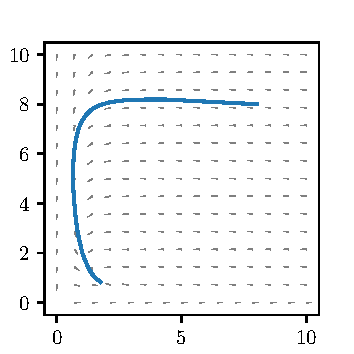
\includegraphics{plots/dynamics.pdf}
\end{figure}
The direction of the flow with optimal behavior (\Cref{fig:pp}(B)) is consistent with the usual Rosenzweig-MacArthur system (\Cref{fig:pp}(A)). The phase portrait reveals that the system dynamics have been stabilized. Looking at the sample trajectory, the system has been overdamped. The stable dynamics stand in contrast to the Rosenzweig-MacArthur model with constant behavior $(\sigma_p=\sigma_c=1)$ where the point of the Hopf bifurcation has been passed, leading to limit cycles.


\begin{figure}[H]
  \label{fig:pp}
  \caption{Transient strategies of consumers $(A)$ and predators $(B)$ at carrying capacity of $K=40$ and a competition of $c=0$ corresponding to the phase portrait \Cref{fig:dynamics}.}
  \label{fig:dynamic_strategies}
  \includegraphics{plots/dynamic_strats.pdf}
\end{figure}
Both consumer and predator strategies change rapidly at the start of the time-interval, before stabilizing towards the equilibrium values. It appears that the consumers are more present in the most productive area when the predator population is lower, which is not that surprising.

\subsection{Population at equilibrium}
\begin{figure}[H]
  \caption{Panel $(A)$ shows population levels of consumers (blue) and predators (red) at equilibrium with changing carrying capacity $(K)$. Panel $(B)$ again shows the population levels, but with varying intraspecific predator competition $(C)$.}
  \label{fig:pop_levels}
  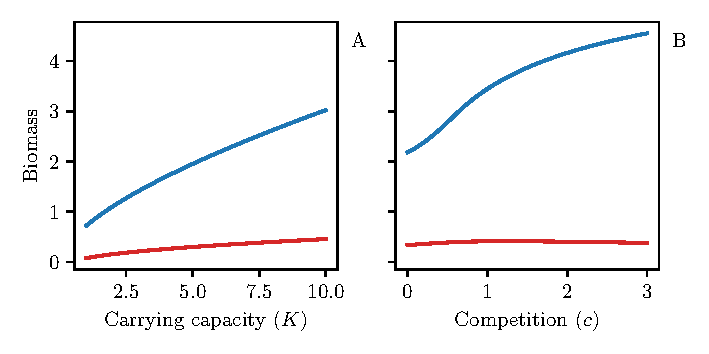
\includegraphics{plots/pop_levels_c.pdf}
\end{figure}
\Cref{fig:pop_levels} reveals how the population levels of consumers and predators change at equilibrium with varying carrying capacity (\Cref{fig:pop_levels}(A)) and intraspecific predator competition (\Cref{fig:pop_levels}(B)).


A higher carrying capacity causes higher populations of both consumers and predators populations at equilibrium (\Cref{fig:pop_levels}). The increase in both populations is probably because the behavioral choice allows the consumers to avoid the risk of predation, while achieving the same fitness.

Varying the intraspecific predator competition causes an increase in the population of predators (\Cref{fig:pop_levels}(C, red)) until a point where the population stabilizes (\Cref{fig:pop_levels}($c\approx 1/3$)). The population of consumers continues to increase (\Cref{fig:pop_levels}(C, blue)) throughout.


\subsection{Spatial distributions}
We start by investigating the spatial distribution of consumers and predators compared to their spatially varying fitness.
\begin{figure}[H]
  \caption{Spatial distribution and fitness of consumers $(A)$ and predators $(B)$ at the equilibrium with carrying capacity $K = 3$.}
  \label{fig:snapshot}
  \includegraphics{plots/snapshot_c.pdf}
\end{figure}
%\Cref{fig:strat_car})
Both consumers and predator distributions have a complex relationship to the fitness levels in the area with co-existence. In the area where there are only consumers, we recognize the emergence of the ideal free distribution. The consumers have a constant fitness level, yet varying concentrations. 

\begin{figure}[H]
  \caption{Spatial distribution of consumers $(A)$ and predators $(B)$ at the equilibrium with increasing carrying capacity $(K)$.}
  \label{fig:strat_car}
  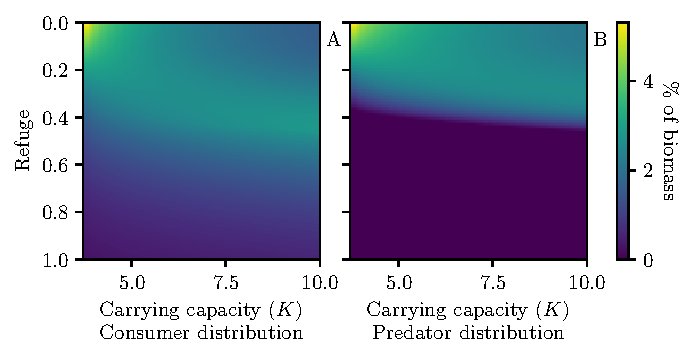
\includegraphics{plots/increasing_car_cap_c.pdf}
\end{figure}
%\Cref{fig:strat_car}) illustrate the strategies of the consumers (\Cref{fig:strat_car}(A)) and predators (\Cref{fig:strat_car}) at equilibrium when carrying capacity varies.

At low carrying capacity consumers are relatively spread out in the most optimal part of the habitat (0-0.3), while predators are concentrated near the most optimal part (0). As the carrying capacity increases, the distribution of consumers becomes more concentrated, distributed around a peak of $0.4$. The peak slowly moves downward with increasing carrying capacity. The consumers can be found throughout the habitat, even at the points of lowest productivity.


Predators go from being concentrated to very spread out, but surprisingly the peak of the predator distribution is just above the peak of the consumer distribution. There are no predators below the band of highly concentrated consumers. This is quite surprising since they have a non-zero encounter rate everywhere. The predator and consumer distributions follow each other as the carrying capacity increases, and appear to approach a stable asymptote.



 %Thus the gain from clustering gradually outweighs the loss from the intraspecific predator competition. That both predator and consumer population increase must be the driving factor behind the peak population concentration moving to less productive areas.

%A higher carrying capacity leads to more concentrated populations, but the increase in populations leads to greater risk-aversion from the consumers so they concentrate in less desirable zones.

\begin{figure}[H]
  \caption{Distribution of consumers $(A)$ and predators $(B)$ at equilibrium under changing predator competition $(c)$.}
  \label{fig:strat_comp}
    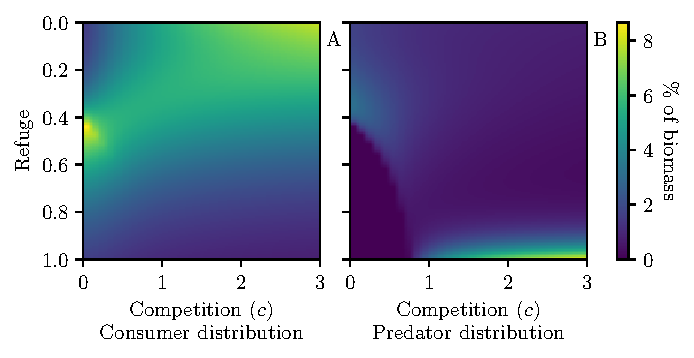
\includegraphics{plots/increasing_competition_c.pdf}
\end{figure}
%In \Cref{fig:strat_comp} the intraspecific predator competition is varied and we see the emergent  equilibrium strategy of the consumers (\Cref{fig:strat_comp}(A)) and predators (\Cref{fig:strat_comp}(B)).

When there is no intraspecific predator competition consumers are highly concentrated at about 0.4, while the predator distributions spreads from 0.4 to 0. The distribution of predators spreads out as we increase competition, before concentrating in the safest zone (1) again. The foraging benefits from clustering on the consumers is outweighed by the risk of encountering other predators. The movement of predators is echoed by the consumers. The consumers spread out and gradually migrate to the most productive area (0). The spreading out of the consumer population though the predator population is concentrated far away is caused by the interspecific competition between consumers, akin to the ideal free distribution. It appears that both consumer and predator densities are converging to asymptotic densities. %An increase in consumer population \Cref{fig:pop_levels} causes an increase in concentration on the less productive spots. When the consumer population spreads out, the distribution trends towards the more productive layers.

\begin{comment}
\begin{figure}[H]
  \caption{Consumer (A) and predator (B) concentration at equilibrium as a function of changing refuge quality}
  \label{fig:ref_qual}

    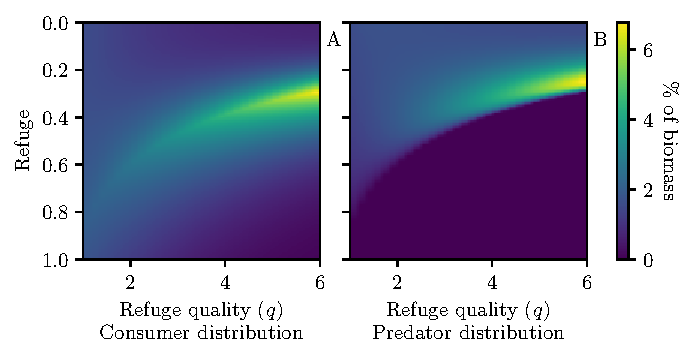
\includegraphics{plots/increasing_refuge_quality_c.pdf}
\end{figure}
\Cref{fig:ref_qual} shows the strategy of consumers (\Cref{fig:ref_qual}(A)) and predators (\Cref{fig:ref_qual}(B)) at equilibrium with varying refuge quality.
\end{comment}

\section{Discussion and conclusion}

We study study population games, based on optimizing individual growth, modifying the definition of \citep{vincent2005evolutionary}. This is done through the introduction of mean-field games, which we show generalizes the ideal free distribution \citep{fretwell1969territorial}. We demonstrate that assuming a monomorphic population is not a viable alternative to the mean-field approach. We do this by showing that the pr. capita payoff a monomorphic population is twice what could be expected from playing the field  \citep{parker1978searching} . Hence, though a population of animals may all be indistinguishable, and appear to follow the same behavioral strategy, it is important to consider how this monomorphism emerges.

We establish existence and uniqueness of Nash equilibria for a large class of games using variational inequalities. In particular, we are able to handle continuous strategy spaces. Having determined existence and uniqueness of Nash equilibrium for the instantaneous game, we showed the existence of fixed-points for suitably nice population games. This provides a simple criterion giving existence and uniqueness for population games, extending theorems based on specific models \citep{cressman2010ideal,sandholm2010population}. Our focus has been on population games, but the results on existence and uniqueness of Nash equilibria are generally applicable to games in biology.

By using our general results, we can show existence and uniqueness of Nash and population equilibria of a Rosenzweig-MacArthur model with behavior in a continuous habitat. This illustates that the problem of showing uniqueness and existence of equilibria for complex population games is feasible, such as \cite{pinti2019trophic}.


After showing existence and uniqueness, we analyzed the modified Rosenzweig-MacArthur game numerically by discretizing space. Adding behavior stabilized the population dynamics, but we have been unable to show analytically why this stability emerges. A possible of attack  for this could be drawing on the theory of complementarity-constrained dynamical systems \citep{adly2018variational,brogliato2020dynamical}. %Skriv noget om sensitvities analysen?


We have not touched on the topic of differential games, where the payoff function for an individual depend on e.g. the entire life history. We expect that the use of variational inequalities and complementarity problems can be extended to differential games. For instance by using Pontryagins maximum principle and approaching the game as a differential variational inequalities \citep{pang2008differential}. Alternatively, the Nash equilibrium can be found explicitly in using backwards time-stepping for for the Hamilton-Jacobi-Bellman equation.

  %We show the framework of mean-field games is applicable in ecology through multi-species population games with optimal individual behavior. We establish theoretical results for existence and uniqueness of Nash equilibria with continuous strategy spaces.

%The payoff for an individual in a large population of indistinguishable individuals is shown much higher when all individuals are a-priori assumed to follow the same strategy.



%We show that a behavorially modified Rosenzweig-MacArthur model has a unique equilibrium by drawing on the general theory we developed. This opens up for sensitivity analysis of the Rosenzweig-MacArthur with respect to the carrying capacity, and the intraspecific predator competition. This analysis is facilitated by a numerical approach based on complementarity. Posing the problem as a complementarity problem changes an optimization problem into a feasibility problem, which is handily solved by IPOPT using the HSL subroutines. The runtimes were impressive, even with a discretization with several hundred grid points.





%KKT can be reformulated as VI, developed by stampacchia mangasarian goeleven et al
%VI solvable numerically, NE existence gives that minimum exists and is 0
%Wide class of VI unique solution, applicable?
%Write up equations for two players, remark that the same for N

%\begin{enumerate}
%  \item What did we find?
%    Highlighted difference between individual and group-level Optimization
%    Concrete calculations showing that individual optimization is less efficient than group level
%    Showed existence and uniqueness of Nash equilibrium
%    Showed existence and uniqueness of population game equilibrium
%    Demonstrted on behavorially modified Rosenzweig-MacArthur model
%    Fast and efficient numerical approach
%  \item What do our results mean?
%    we now have good criteria for uniqueness and existence, less ad-hoc.%
    %Behavior can become the norm.
    %Models need to look at the individual perspective rather than population level.
    %Illustrates the difference between emergent monomorphism and inherent monomorphism
    %Selfish behavior is much less advantageous for the collective

%  \item Perspectives in VI for NE in ecology  Compare to literature also the stuff by Patrizio. remark well-known that worse for species than population-thingy
%    Fast numerics can be implemented by anynone, for a fairly general set of games not just related to populations
%    Feasible to implemement population games generally, behavior can be as much of a choice as seasons
%    Realistic models of ecosystems
%    The work is hinted at in the work of Sandholm, but not developed further.
%    We focus on continuous, but much stronger results actually hold in finite habitat choice setting.
%    It has become possible to include bona-fide continuous habitats.
%  \item
%    Games with long-term optimization can be implemented as differential variational inequalities
%    Multiple species in actual Applications
%    Check the Scalability
%    Try wtih dedicated software, see how fast it can get.
%
%\end{enumerate}



%\begin{acknowledgements}
%I would like to thank my supervisor Uffe H. Thygesen for fruitful discussions during the development of the model and the initial studies on static mean-field games.
%\end{acknowledgements}


% Authors must disclose all relationships or interests that
% could have direct or potential influence or impart bias on
% the work:
%
% \section*{Conflict of interest}
%
% The authors declare that they have no conflict of interest.
\subsection*{Declarations}

\subsubsection*{Funding}
This work was supported by the Centre for Ocean Life,
a Villum Kann Rasmussen Centre of Excellence supported
by the Villum Foundation.
\subsubsection*{Code availability}
All code for reproducing the results of this project is available on github \url{https://github.com/jemff/MFG_Static}.
\subsubsection*{Conflict of interest}
The authors declare that they have no conflict of interest.
\subsubsection*{Authors' contributions}
E.F.F. designed the study. E.F.F. realized the model design E.F.F. coded the model and chose the numerical approach. E.F.F. analyzed the results along with U.H.T.. E.F.F. wrote the paper. All authors read and approved the final version.
\subsubsection*{Data availability}
All data can be generated using the files 2d_sensitivity.py and phase_wrapper.py at \url{https://github.com/jemff/MFG_Static}.
% BibTeX users please use one of
\bibliographystyle{spbasic}      % basic style, author-year citations
%\bibliographystyle{spmpsci}      % mathematics and physical sciences
%\bibliographystyle{spphys}       % APS-like style for physics
\bibliography{bibliography}   % name your BibTeX data base

\appendix
\section{Results on variational inequalities}
\label{sec:appendix}
The following section contains the necessary results on variational inequalities, which have been removed from the main text to improve the flow.

We start by recalling the definition of pseudo-convexity
The corresponding notion of convexity is
\begin{definition}
  Let $\Omega \subset H$ be an open subset of $H$, and let $f:\Omega \to \R$ be Gateaux-differentiable. The function $f$ is strictly pseudoconvex if
  \begin{equation}
    \ip{y-x}{(\nabla f)(x)} \geq 0 \Rightarrow f(y) > f(x)
  \end{equation}
\end{definition}
Where a strictly convex function has a strictly monotone derivative, a variant holds for strictly pseudoconvex functions. First, we need to introduce strict pseudomonotonicity.
\begin{definition}
 The operator $T: K \to H$ is strictly pseudomonotone if for every pair $x\neq y$ we have
 \begin{align}
   \ip{x-y}{Ty} \geq 0 \Rightarrow \ip{x-y}{Tx} > 0
 \end{align}
\end{definition}
Proving strict pseudomonotonicity in itself can be hard, but thankfully the notions of strict pseudomonotonicity and strict pseudoconvexity are related.
\begin{theorem}[Theorem 12.13, p. 521 \citep{hadjisavvas2006handbook}]
  Let $\Omega \subset H$ be an open convex subset, and let $f:\Omega \to \R$ be Gateaux differentiable. Then $f$ is strictly pseudoconvex if and only if $\nabla f$ is strictly pseudomonotone.
\end{theorem}
Minimizing a differentiable strictly pseudoconvex $f$ function over a convex set $K$ is equivalent to solving the variational inequality
\begin{equation}
  x \in K, ~ \ip{(\nabla f)(x)}{x-y} \geq 0, \forall y\in K
\end{equation}
The problem of existence and uniqueness of a Nash equilibrium has been reduced to a problem of existence and uniqueness of a variational inequality. Whether a variational inequality given by a pseudomonotone operator has a solution can be determined by \citep[Theorem 3.4]{maugeri2009existence}, which we abridge:
\begin{theorem}
  \label{thm:existence}
  Let $K$ be a closed convex set and $A : K \to H$  a pseudo-
  monotone map which is continuous on finite dimensional subspaces of $H$. Then the fol-
  lowing statements are equivalent:
\end{theorem}
\begin{enumerate}
  \item The variational inequality $\ip{Ax}{y-x} \geq 0$ admits solutions.
  \item There exists a point $u_0 \in K$ such that the set
  \begin{equation}
    \{v \in K : \ip{A(v)}{v-u_0} < 0\}
  \end{equation}
  is bounded.
\end{enumerate}
We also state another characterization of strict pseudomonotonicity for differentiable functions, since this criterion is easier to check in practice than going to the definition.
  \begin{lemma}
  \label{lem:strict_pm}
  Let $K$ be a convex subset of $H$. A function $f: K \to \R$ is strictly pseudomonotone if
  \begin{equation}o
    \ip{f(x)}{u} = 0 \Rightarrow \ip{(\nabla_x f(x))h}{h} > 0
  \end{equation}
\end{lemma}
A proof can be found in \citep[Proposition 2.8, p.96]{hadjisavvas2006handbook}

\begin{comment}

\citep[Theorem 3.6]{maugeri2009existence}, which we restate.
\begin{theorem}
  \label{thm:existence}
  Let $K\subset H$ be a closed convex set and $T:K\to H$ a pseudomonotone operator which is lower hemicontinuous along line segments, i.e. for all $x,y\in H$ the mapping $\xi \mapsto \ip{T\xi,}{x-y}$ is lower semicontinuous for $\xi \in \{\eta \in H : \eta = tx+(1-t)y, \quad t\in [0,1]\}$. Assume that there exists $u_0 \in K$ and $R> \norm{u_0}$ such that
  \begin{equation}
    \ip{Tv}{v-u_0} \geq 0, \forall v \in K \cap \{v \in H : \norm{v} = R \}
  \end{equation}
  then the variational inequality $VI(T,K)$ has a solution.
\end{theorem}
\end{comment}
\begin{remark}
  \label{rem:weak_compact}
  Weak compactness of $K$ also ensures that $VI(T,K)$ has a solution \citep[Theorem 12.1, P. 510]{hadjisavvas2006handbook}, giving existence of solutions in the finite-dimensional case.
\end{remark}
With a criterion for existence in hand, we proceed to state a criterion for uniqueness, justifying our focus on strict pseudoconvexity and strict pseudomonotonicity.
\begin{theorem}[Lemma 12.3, p. 516, \citep{hadjisavvas2006handbook}]
  \label{thm:uniqueness}
  Let $K\subset H$ be a non-empty subset of $H$. If $T$ is strictly pseudomonotone, then the problem $VI(T,K)$ has at most one solution.
\end{theorem}
\subsection{Calculations}
\label{appendix:calculations}
We complete the omitted calculations from the main text. Computing
\begin{equation}
  \ip{dU(\sigma_c,\sigma_p)}{(\sigma_c-1, \sigma_p-1)} =
\end{equation}

%\appendix
%\section{Results on variational inequalities}
\label{sec:appendix}
The following section contains the necessary results on variational inequalities, which have been removed from the main text to improve the flow.

We start by recalling the definition of pseudo-convexity
The corresponding notion of convexity is
\begin{definition}
  Let $\Omega \subset H$ be an open subset of $H$, and let $f:\Omega \to \R$ be Gateaux-differentiable. The function $f$ is strictly pseudoconvex if
  \begin{equation}
    \ip{y-x}{(\nabla f)(x)} \geq 0 \Rightarrow f(y) > f(x)
  \end{equation}
\end{definition}
Where a strictly convex function has a strictly monotone derivative, a variant holds for strictly pseudoconvex functions. First, we need to introduce strict pseudomonotonicity.
\begin{definition}
 The operator $T: K \to H$ is strictly pseudomonotone if for every pair $x\neq y$ we have
 \begin{align}
   \ip{x-y}{Ty} \geq 0 \Rightarrow \ip{x-y}{Tx} > 0
 \end{align}
\end{definition}
Proving strict pseudomonotonicity in itself can be hard, but thankfully the notions of strict pseudomonotonicity and strict pseudoconvexity are related.
\begin{theorem}[Theorem 12.13, p. 521 \citep{hadjisavvas2006handbook}]
  Let $\Omega \subset H$ be an open convex subset, and let $f:\Omega \to \R$ be Gateaux differentiable. Then $f$ is strictly pseudoconvex if and only if $\nabla f$ is strictly pseudomonotone.
\end{theorem}
Minimizing a differentiable strictly pseudoconvex $f$ function over a convex set $K$ is equivalent to solving the variational inequality
\begin{equation}
  x \in K, ~ \ip{(\nabla f)(x)}{x-y} \geq 0, \forall y\in K
\end{equation}
The problem of existence and uniqueness of a Nash equilibrium has been reduced to a problem of existence and uniqueness of a variational inequality. Whether a variational inequality given by a pseudomonotone operator has a solution can be determined by \citep[Theorem 3.4]{maugeri2009existence}, which we abridge:
\begin{theorem}
  \label{thm:existence}
  Let $K$ be a closed convex set and $A : K \to H$  a pseudo-
  monotone map which is continuous on finite dimensional subspaces of $H$. Then the fol-
  lowing statements are equivalent:
\end{theorem}
\begin{enumerate}
  \item The variational inequality $\ip{Ax}{y-x} \geq 0$ admits solutions.
  \item There exists a point $u_0 \in K$ such that the set
  \begin{equation}
    \{v \in K : \ip{A(v)}{v-u_0} < 0\}
  \end{equation}
  is bounded.
\end{enumerate}
We also state another characterization of strict pseudomonotonicity for differentiable functions, since this criterion is easier to check in practice than going to the definition.
  \begin{lemma}
  \label{lem:strict_pm}
  Let $K$ be a convex subset of $H$. A function $f: K \to \R$ is strictly pseudomonotone if
  \begin{equation}o
    \ip{f(x)}{u} = 0 \Rightarrow \ip{(\nabla_x f(x))h}{h} > 0
  \end{equation}
\end{lemma}
A proof can be found in \citep[Proposition 2.8, p.96]{hadjisavvas2006handbook}

\begin{comment}

\citep[Theorem 3.6]{maugeri2009existence}, which we restate.
\begin{theorem}
  \label{thm:existence}
  Let $K\subset H$ be a closed convex set and $T:K\to H$ a pseudomonotone operator which is lower hemicontinuous along line segments, i.e. for all $x,y\in H$ the mapping $\xi \mapsto \ip{T\xi,}{x-y}$ is lower semicontinuous for $\xi \in \{\eta \in H : \eta = tx+(1-t)y, \quad t\in [0,1]\}$. Assume that there exists $u_0 \in K$ and $R> \norm{u_0}$ such that
  \begin{equation}
    \ip{Tv}{v-u_0} \geq 0, \forall v \in K \cap \{v \in H : \norm{v} = R \}
  \end{equation}
  then the variational inequality $VI(T,K)$ has a solution.
\end{theorem}
\end{comment}
\begin{remark}
  \label{rem:weak_compact}
  Weak compactness of $K$ also ensures that $VI(T,K)$ has a solution \citep[Theorem 12.1, P. 510]{hadjisavvas2006handbook}, giving existence of solutions in the finite-dimensional case.
\end{remark}
With a criterion for existence in hand, we proceed to state a criterion for uniqueness, justifying our focus on strict pseudoconvexity and strict pseudomonotonicity.
\begin{theorem}[Lemma 12.3, p. 516, \citep{hadjisavvas2006handbook}]
  \label{thm:uniqueness}
  Let $K\subset H$ be a non-empty subset of $H$. If $T$ is strictly pseudomonotone, then the problem $VI(T,K)$ has at most one solution.
\end{theorem}
\subsection{Calculations}
\label{appendix:calculations}
We complete the omitted calculations from the main text. Computing
\begin{equation}
  \ip{dU(\sigma_c,\sigma_p)}{(\sigma_c-1, \sigma_p-1)} =
\end{equation}

% Non-BibTeX users please use
%\begin{thebibliography}{}
%
% and use \bibitem to create references. Consult the Instructions
% for authors for reference list style.
%
%\bibitem{RefJ}
% Format for Journal Reference
%Author, Article title, Journal, Volume, page numbers (year)
% Format for books
%\bibitem{RefB}
%Author, Book title, page numbers. Publisher, place (year)
% etc
%\end{thebibliography}

\end{document}
% end of file template.tex
